\chapter{Aplicação exemplar com arquitetura de microsserviços}\label{chapter-aplicacao}

\chapterprecis{Este capítulo apresenta a aplicação exemplar com arquitetura de microsserviços desenvolvida.}\index{sinopse de capítulo}


A aplicação desenvolvida trata-se de um sistema web de e-commerce. Nela, um cliente da loja pode buscar e comprar produtos, enquanto um administrador pode gerenciar produtos e usuários cadastrados, tudo a partir de uma interface de usuário em um navegador.
O código fonte está disponível no repositório do GitHub com link \url{https://github.com/Jp9910/microservices_project}

Os diagramas de classes, pacotes e componentes podem ser vistos na \autoref{figura-diagrama-de-classes}, \autoref{figura-diagrama-de-pacotes} e \autoref{figura-diagrama-de-componentes}, respectivamente.

\section{Divisão dos microsserviços}
% TODO: diagramas de classes, de pacotes, e de sequencia dos microsserviços

[EM PROGRESSO] Foram usados conceitos do domain-driven design para determinar os limites de cada microsserviço...

Falar sobre o Padrão MVC, CLEAN architecture e SOLID principles usados nos microsserviços

[EM PROGRESSO] Em especial houve uma dúvida muito grande quanto a qual microsserviço será responsável pela lógica de negócios dos pedidos e seu armazenamento. Foram considerados o microsserviço de carrinho (que viraria o microsserviço de pedidos) ou o microsserviço de loja (que sem os pedidos viraria o microsserviço de catálogo). No fim decidi implementar no microsserviço de loja porque...

\subsection*{Serviço de negócios - Loja}
Esse microsserviço trata da lógica de negócios relacionada a produtos e pedidos.

\subsection*{Serviço de negócios - Carrinho}
Esse microsserviço trata da lógica de negócios relacionada ao carrinho e realização da compra.

\subsection*{Serviço de negócios - Usuários}
Esse microsserviço trata da lógica de negócios relacionada ao cadastro e autenticação de usuários.

\subsection*{Serviço de negócios - Financeiro}
Esse microsserviço trata apenas do processamento (fictício) do pagamento de um pedido.

\subsection*{Serviço de ponta - Clientes}
O microsserviço de ponta de clientes é o serviço acessado diretamente pelos clientes da loja para realizar todas as operações relevantes a eles a partir de uma interface de usuário, tal como ver e buscar produtos, adicionar produtos ao carrinho e realizar um pedido a partir de um carrinho.

\subsection*{Serviço de ponta - Administração}
O microsserviço de ponta de administração é o serviço usado pelos administradores da loja para realizar todas as operações relevantes a eles a partir de uma interface de usuário, tal como gerenciar produtos e usuários.


\begin{figure}[htb]
	\caption{\label{figura-diagrama-de-classes}Diagrama de classes da aplicação exemplar}
	\begin{center}
	    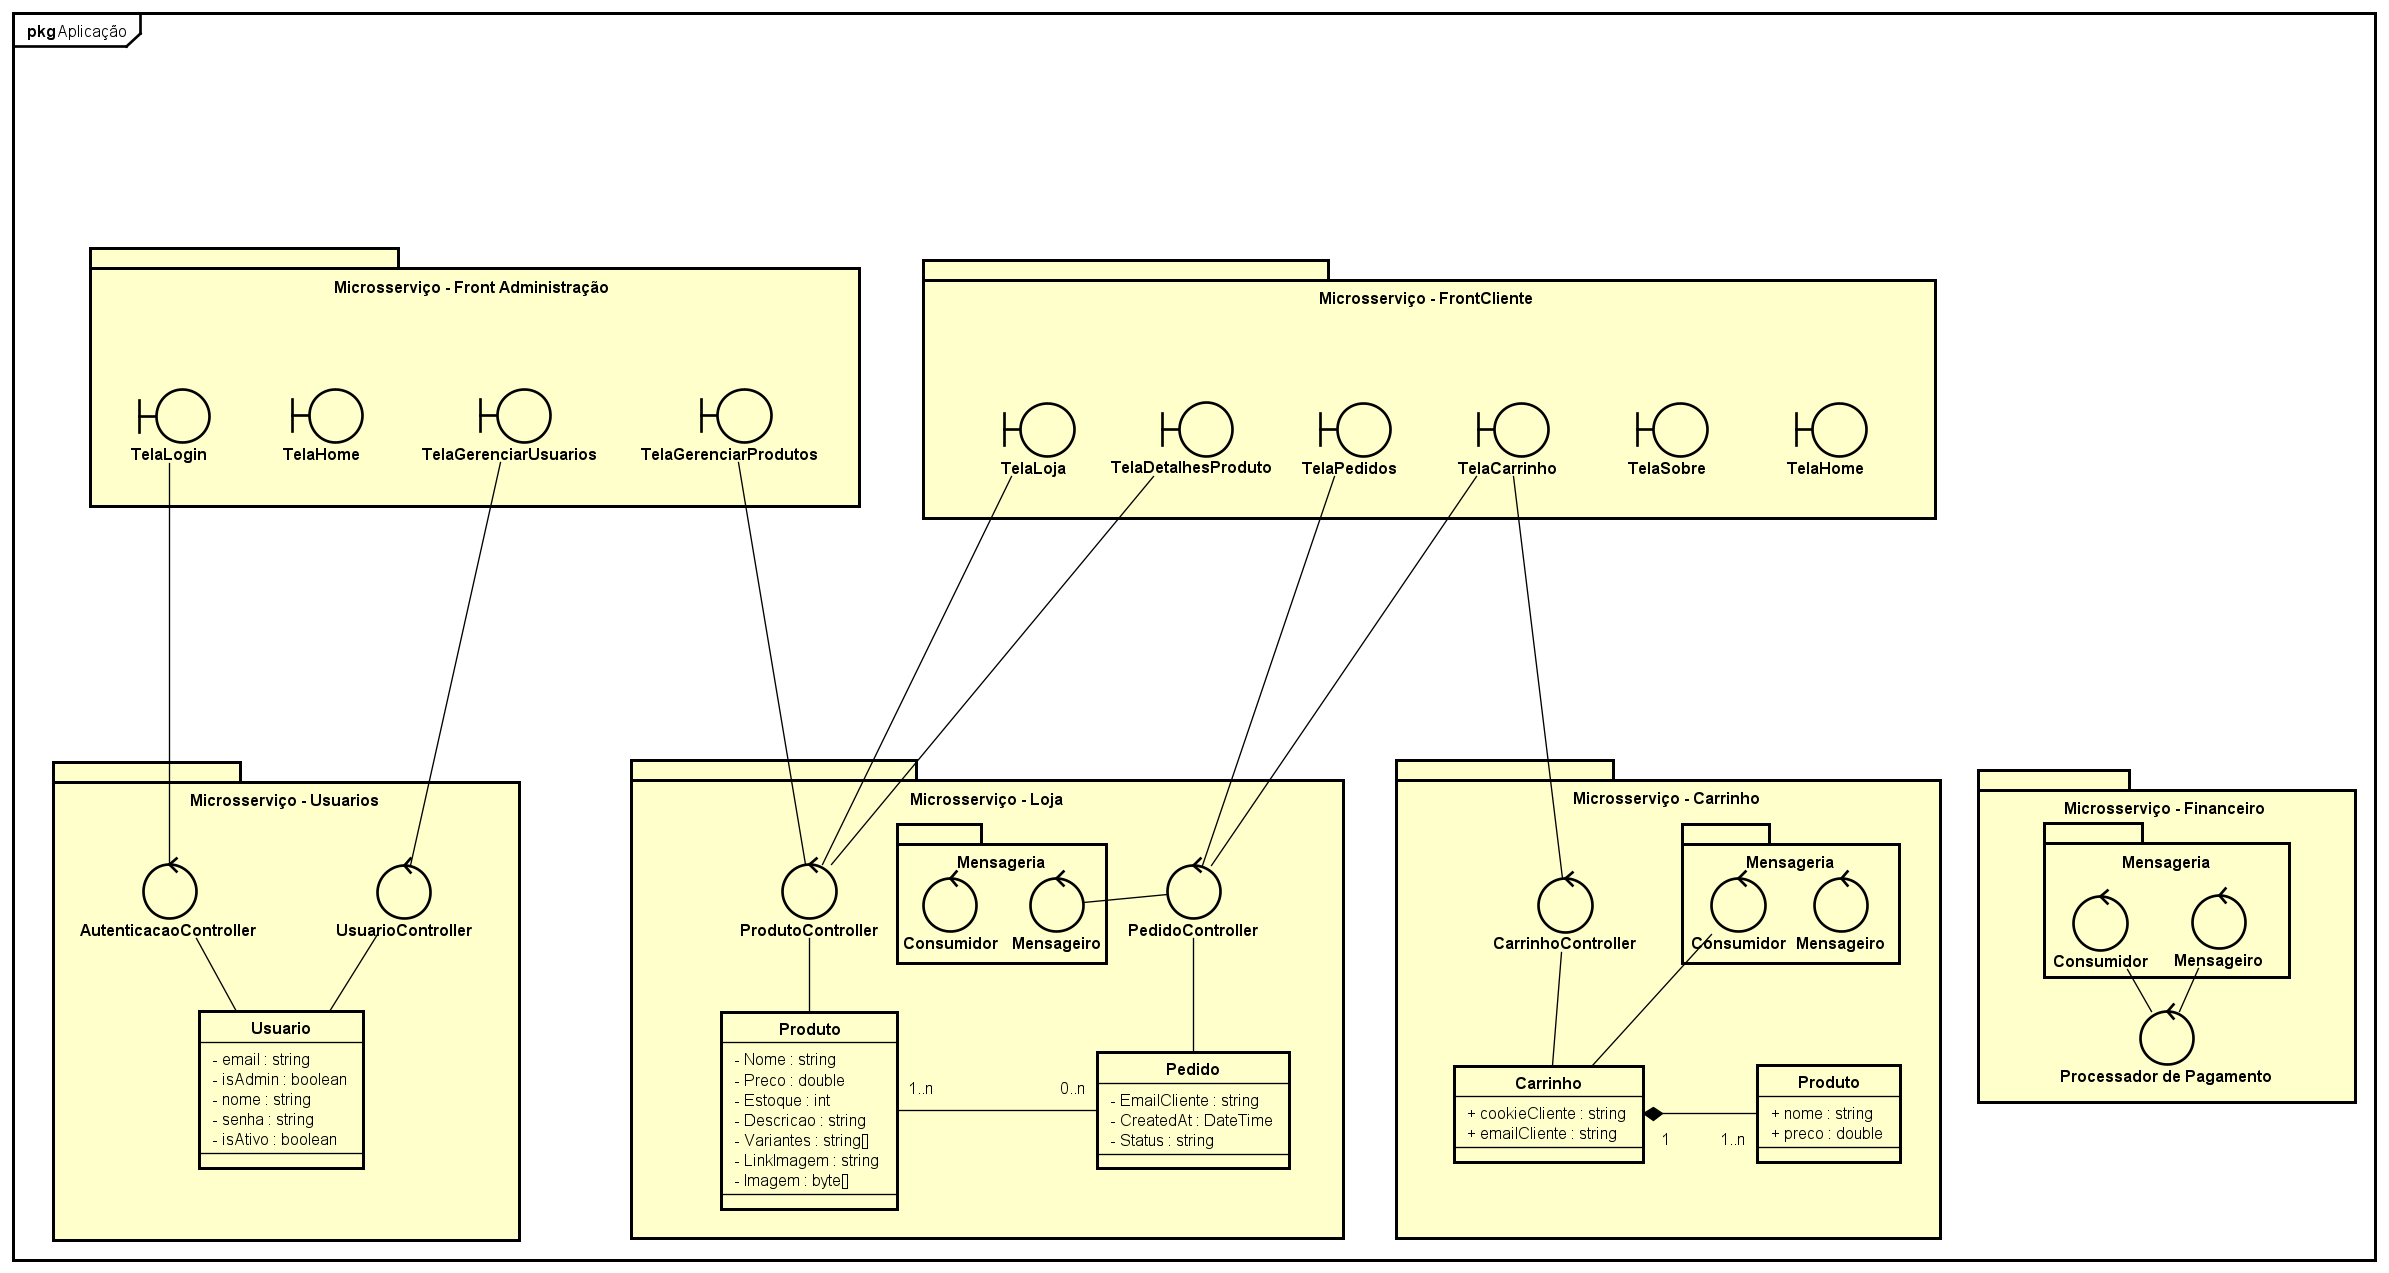
\includegraphics[scale=0.25]{Diagramas/imagens/Classes.png}
	\end{center}
	\legend{Fonte: Autor}
\end{figure}

\begin{figure}[htb]
	\caption{\label{figura-diagrama-de-pacotes}Diagrama de pacotes da aplicação exemplar}
	\begin{center}
	    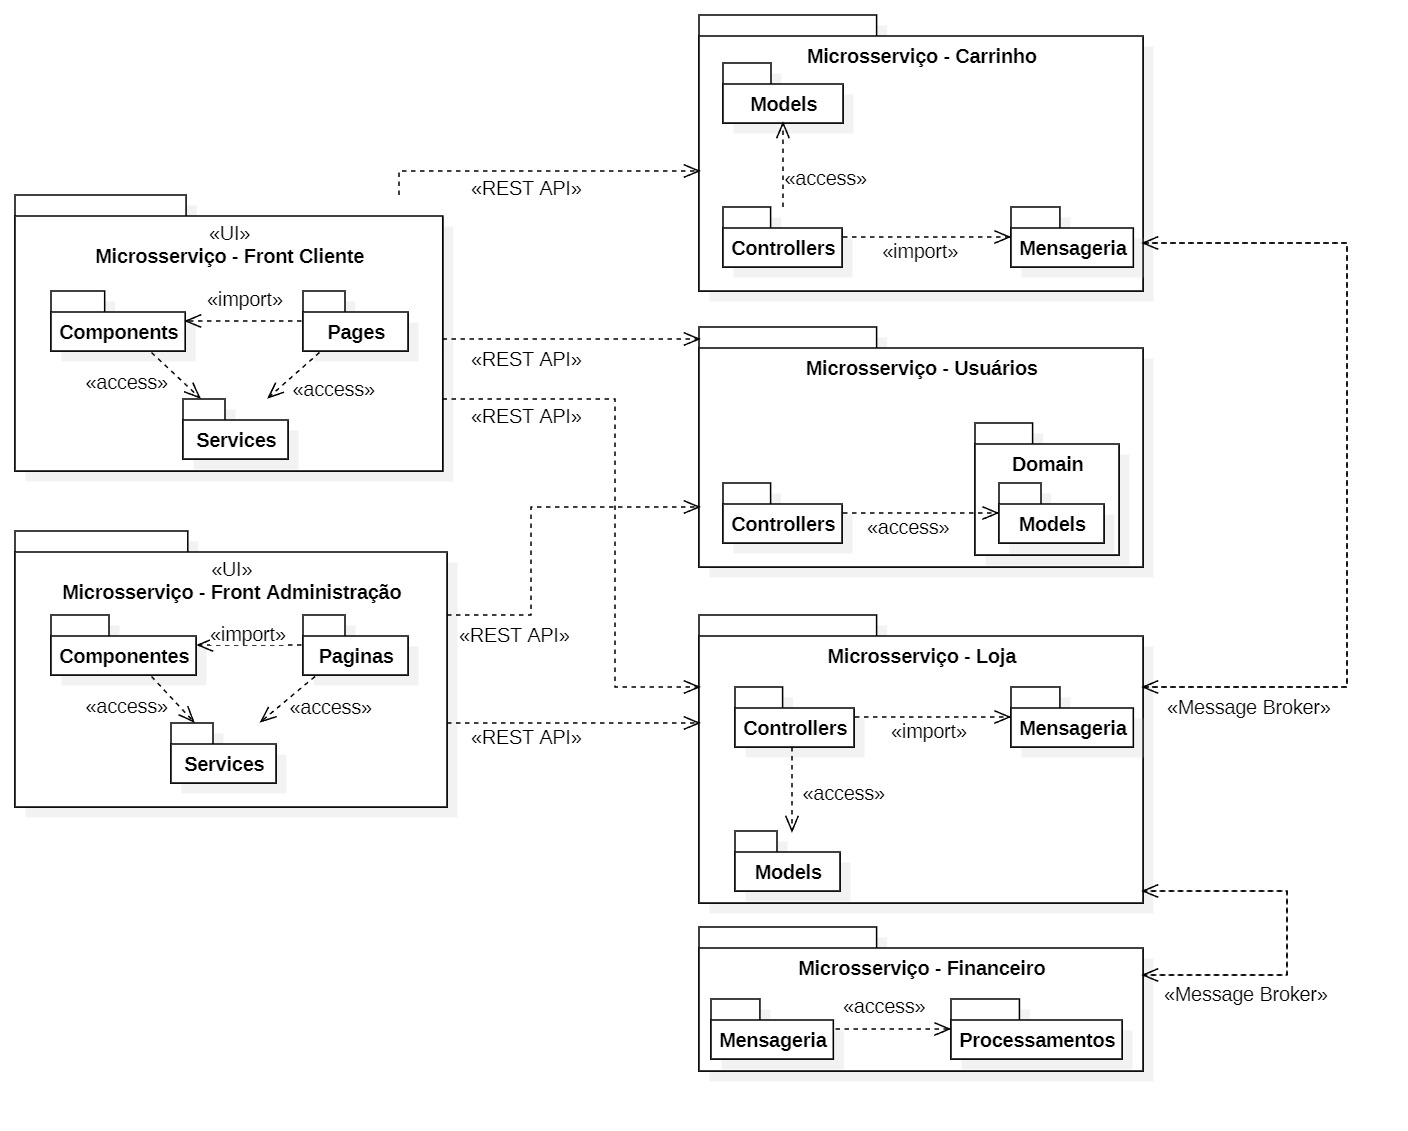
\includegraphics[scale=0.27]{Diagramas/imagens/Pacotes.jpg}
	\end{center}
	\legend{Fonte: Autor}
\end{figure}

\begin{figure}[htb]
	\caption{\label{figura-diagrama-de-componentes}Diagrama de componentes da aplicação exemplar}
	\begin{center}
	    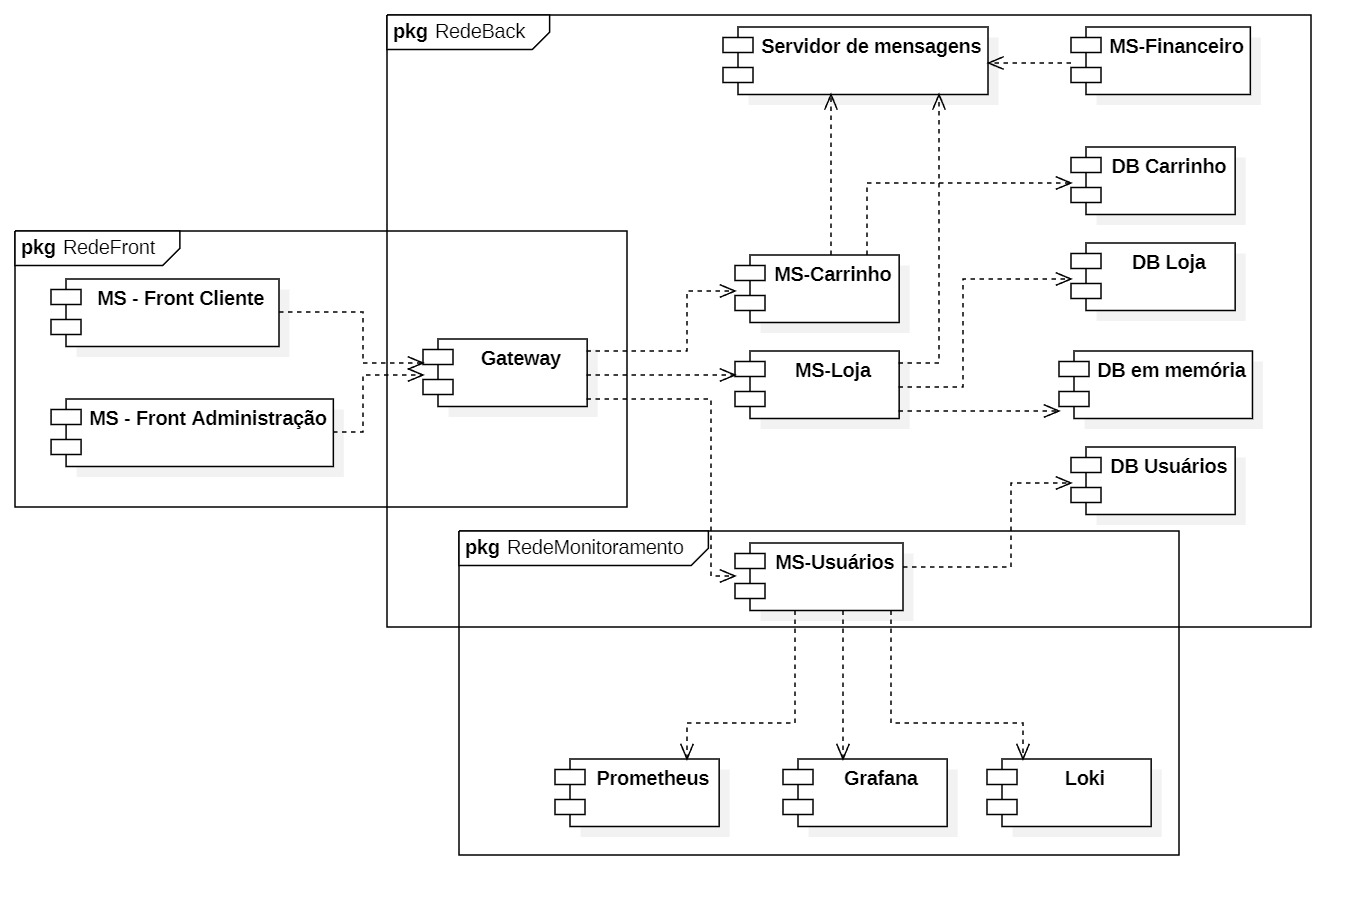
\includegraphics[scale=0.27]{Diagramas/imagens/Componentes-Redes.jpg}
	\end{center}
	\legend{Fonte: Autor}
\end{figure}

\begin{figure}[htb]
	\caption{\label{figura-diagrama-de-sequencia}Diagrama de sequência de fazer uma compra no carrinho}
	\begin{center}
	    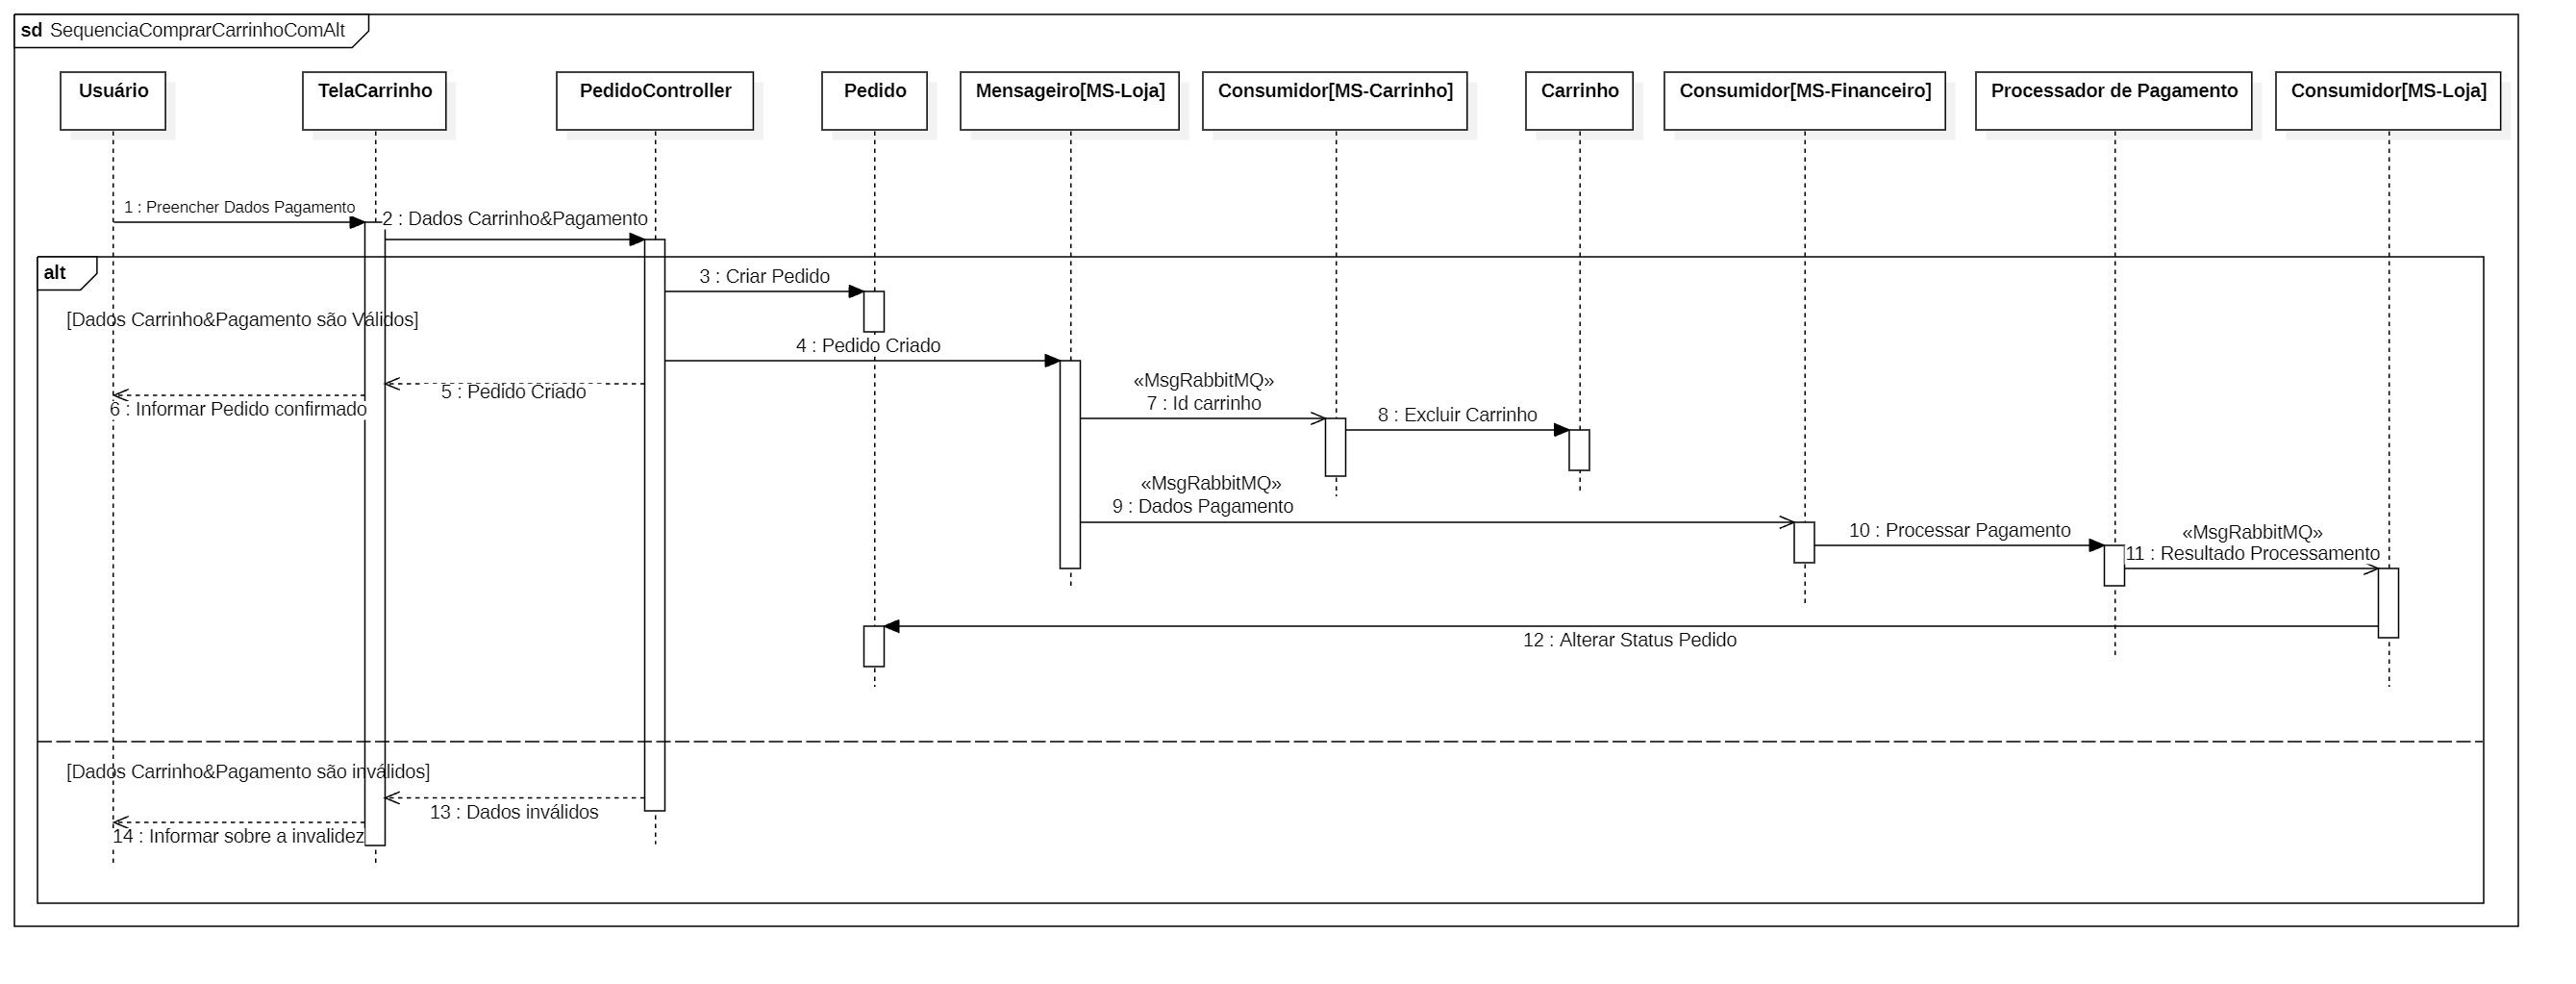
\includegraphics[scale=0.16]{Diagramas/imagens/SequenciaComprarCarrinhoComAlt.jpg}
	\end{center}
	\legend{Fonte: Autor}
\end{figure}


\section{Práticas e ferramentas usadas}
\subsection*{\emph{Frameworks} e linguagens de programação}
Para demonstrar a flexibilidade da arquitetura de microsserviços e como oportunidade para aprender novos \emph{frameworks}, foram usados diferentes \emph{frameworks} e linguagens de programação para os microsserviços. O microsserviço de usuários foi feito com Java e Spring Boot, o de loja com C\# e .NET, o de carrinho e de financeiro com TypeScript e ExpressJS, o de ponta de cliente com ReactJS e o de ponta de administração com Angular.

\subsection*{Servidor web e Gateway}
Como servidor web foi usado o Nginx nos serviços de ponta para servir os arquivos estáticos, por ser simples de configurar e oferecer diversas funcionalidades proveitosas para microsserviços. Além disso, ele também foi usado no componente de Gateway como um API Gateway para o intermédio da comunicação entre os serviços de ponta e os serviços de negócio, redirecionando as requisições dos serviços de ponta para os serviços de negócio apropriados.

\subsection*{Bancos de dados e descentralização dos dados}
Foram usados diferentes instâncias e tecnologias de bancos de dados na aplicação desenvolvida, assim proporcionando a descentralização dos dados. Nos microsserviços de loja e de usuários foi usado o banco de dados relacional PostgreSQL, tanto pela simplicidade de configuração quanto pela consistência de dados de operações mais importantes, como criação de um pedido ou de um usuário.

No microsserviço de carrinho foi usado o banco de dados NoSQL MongoDB porque um carrinho tem uma estrutura mais dinâmica, com itens podendo ter estruturas diferentes e sendo adicionados, alterados e removidos frequentemente.

Além disso, também foi usado o banco de dados em memória Memcached para realizar o \emph{caching} da busca de produtos no microsserviço de loja, assim proporcionando menor latência e consumo de recurso nessa operação que é executada com alta frequência.

\subsection*{Metodologia 12-fatores}
A maioria dos fatores da \hyperref[metodologia-12-fatores]{metodologia 12-fatores} foram considerados e cumpridos no desenvolvimento da aplicação: I - Base de código única; II - Dependências portáteis e isoladas; III - Externalizar configurações; IV - Serviços de apoio são anexos; V - Separação entre construção, lançamento, e execução; VI - Processos sem estado (os microsserviços de ponta guardam a informação do usuário no navegador do cliente); VIII - simultaneidade; IX - Descartabilidade; X - Paridade de ambientes de execução; XI - \emph{Logs}; e XII - Processos administrativos.

\subsection*{CI/CD}
Foi usado o Git como sistema de controle de versão e o GitHub para gerenciamento de repositórios em todos os microsserviços, com configuração de proteção do ramo principal do repositório para evitar \emph{commits} indevidos, assim sendo necessário a criação de um \emph{pull request} e aprovação dele por um administrador do repositório para integração do novo código no ramo principal. 

No microsserviço de ponta de administração também foi implementado um \emph{pipeline} de CI/CD com 3 etapas sequenciais, com uso do GitHub Actions como servidor de integração para executar o \emph{pipeline} automaticamente a cada novo \emph{commit} recebido. A primeiro etapa executa o \emph{linting} nos arquivos JavaScript com o ESLint e os testes de unidade com a biblioteca Karma; a segunda etapa faz a construção e upload do artefato já com o novo código. A terceira etapa usa esse artefato para criar uma imagem de container Docker pronta para implantação, que é subida para o DockerHub, um repositório publico de imagens Docker, assim podendo ser baixada facilmente em qualquer máquina. 

[anotação] Poderia ter um diagrama mostrando o pipeline
% Deveria ter um print Mostrar o exemplo do pipeline CICD rodando no GitHub Actions, com proteções de branch e requerimento de revisão de código ?


\subsection*{Organização do código - Multirepo}
Para organização do código foi utilizada a técnica Multirepo com os repositórios no GitHub. Cada microsserviço possui um único repositório independente, porém também há um repositório principal que contém referências para os repositórios de cada microsserviço, reunindo tudo que é necessário para executar a aplicação inteira.

\subsection*{Contêinerização e orquestração de contêineres}
[EM PROGRESSO]

Contêirezação com Docker e orquestração com docker-compose para desenvolvimento e Kubernetes para produção

Mencionar sobre a replicação e tudo mais do kubernetes.

O kubernetes vai buscar as imagens do repositório de imagens DockerHub e usá-las para configurar os containers para implantação

As configurações foram externalizadas, favorecendo a portabilidade. Todos os microsserviços podem ser iniciados em modo de desenvolvimento ou produção com mínimas alterações necessárias, apenas sendo necessário definir algumas variáveis de ambiente sensíveis, tal como a senha do banco de dados. Além disso, todos os microsserviços tem configurações de desenvolvimento e produção. Os serviços de ponta por exemplo, já usam essas configurações para definir o endereço dos microsserviços de negócio para onde vão fazer as requisições.

\subsection*{Testes}
[EM PROGRESSO]
Testes de unidade. Selenium?

\subsection*{APIs}
[EM PROGRESSO]

RESTful, 

\subsection*{Comunicação assíncrona}
[EM PROGRESSO] RabbitMQ

\subsection*{Monitoramento}
[EM PROGRESSO] Prometheus, grafana, loki,

O monitoramento foi feito apenas para o microsserviço de usuários por falta de tempo, mas todos os microsserviços podem ser configurados para utilizá-los, e novos \emph{dashboards} podem ser criados para monitorá-los